\documentclass[../main.tex]{subfiles}

\begin{document}
Honeypots are one of the strategies employed in defensive security to detect attacks from adversaries. They are designed and developed with an intention to mimic the real protocols and provide information about the attack to the administrators. Based on the interaction and service emulation, honeypots are classified into low, medium and high interaction honeypots. Security administrators often feel that low interaction honeypots are feasible to be deployed in their environment as they are not resource intensive and are less risky. Low interaction honeypots are limited in protocol emulations and hence are also easy targets for fingerprinting attacks. 

Fingerprinting techniques are used to identify systems by analysis on the behavioral information retrieved by probing. It is normally the first step employed by attackers to gain more insight about the end system before exploiting them. This technique has proved to be effective and there are various fingerprinting tools available that can accurately determine the operating system, kernel versions, protocol versions, device name and other attributes of the end system. However, determining these attribute information may involve multiple scans and intermittent probing. The ideal outcome of device fingerprinting infers the device and its attributes, based on which the attacker can orchestrate exploits. The primary focus of a honeypot lies in its ability to stay undetected. Attackers use fingerprinting as an initial setup to determine the validity of the end device before investing their resources on exploitation. If the identity of honeypot is revealed during the initial fingerprinting techniques, there productivity is degraded. This happens due to two reasons. Firstly, the attacker decides to broadcast his findings about the existence of the honeypot which alerts other attackers when they are looking for targets. Second, there is a derived fingerprinting technique for the target honeypot, which can be included in the primary scan of popular fingerprinting tools. p0f, Nmap, Uniscan, Metasploit, Nikto and cisco-torch are some of the open-source fingerprinting tools which are capable of detecting honeypots like Kippo, Cowrie and Glastopf. Table \ref{tab:Table1} provides a list of protocols and the honeypots available on the internet.   

    \begin{figure}
    \begin{center}
    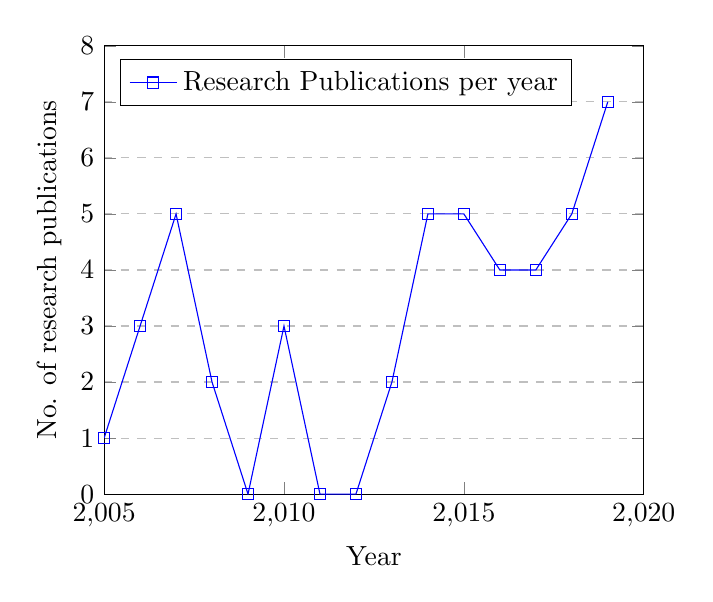
\begin{tikzpicture}
    \begin{axis}[
   %% title={Research on System and Network Fingerprinting},
    xlabel={Year},
    ylabel={No. of research publications},
    xmin=2005, xmax=2020,
    ymin=0, ymax=8,
    xtick={2005,2010,2015,2020},
    ytick={0,1,2,3,4,5,6,7,8},
    legend pos=north west,
    ymajorgrids=true,
    grid style=dashed,
    ]

    \addplot[
    color=blue,
    mark=square,
    ]
    coordinates {
    (2005,1)(2006,3)(2007,5)(2008,2)(2009,0)(2010,3)(2011,0)(2012,0)(2013,2)(2014,5)(2015,5)(2016,4)(2017,4)(2018,5)(2019,7)
    };
    \legend{Research Publications per year}
    
    \end{axis}
    \end{tikzpicture}
    \end{center}
    \caption{Research on System and Network Fingerprinting}
    \label{fig:research_per_year}
   \end{figure} 
    

Identifying deviations in the behavior of a system and inferring fingerprints has been an active research topic. Early works by Brumley et al. \cite{Brumley} involved theoretical approach based on binary analysis. All attacks towards honeypots are recorded or logged for further analysis. This process is an expensive operation considering the writes and file operations thereby creating delay in the response times of the honeypot. Further, honeypots utilize the virtual environments to save resources in their environment. Based on these ideas, Holz et al \cite{Holz} proposed that honeypots could be detected due to increase in execution time of the commands from the attackers because of logging and sandboxing.Fu et al. \cite{Fu} also, suggested that the delay in execution and the response due to the virtualized network layer leveraged by honeypots could be a factor to infer the presence of the honeypot. At the Black Hat conference 2015, Cymmetria research \cite{BLACKHAT} proposed various factors by which honeypots could be fingerprinted and recommended new design strategies and development practices to overcome the detection. Alexander et al. \cite{Vetterl2018} provide a systematic fingerprinting approach for low-interaction honeypots. They leverage the faults of poorly maintained libraries referenced in the emulation of protocols in popular honeypots. The libraries used in the development of protocols in honeypots were not intended to reproduce the actual behavior of the protocol itself but used for the ease of development. The authors present a fingerprinting approach by development of probes that trigger the response at the transport layer and were successful in identifying up to 7605 honeypots online. Their research is limited to SSH, Telnet and HTTP honeypots. Internet scanning tools like Shodan have also released Honeypot identification methods called Honeyscore \cite{SHODAN}.The tool accepts an IP address or a URL as an input and provides result if the end system is a honeypot. The tool is stated to be still in development but is capable of recognizing popular honeypots on the internet. Feng et al. \cite{Feng2016} propose a machine learning model to collect and classify the response data received from Industrial Control Systems open on the internet. The approach relies on the flawed implementation of industrial control protocols and the deployment configurations of the honeypots. Figure \ref{fig:research_per_year} shows the increasing research in the area of system fingerprinting over the years. Over the last five years, there is consistent increase for fingerprinting research techniques. 



\begin{table*}[ht!]
\caption{\label{tab:Table1}Protocols and Honeypots}
\centering
 \begin{tabular}{||c c c c c c c||} 
 \hline
 SSH & Telnet & HTTP & SMB & Database & ICS & IoT\\ [0.5ex] 
 \hline
 Kippo & Telnet-IOT-Honeypot & Dionaea & HoneySMB & mysql-honeypotd & Conpot & HoneyThing\\ 
 
 HosTaGe &  HosTaGe &  HosTaGe &  HosTaGe &  HosTaGe &  HosTaGe &  HosTaGe  \\
 
 Cowrie & Cowrie & Glastopf &  & pghoney & GasPot & Kako\\

 Blacknet & TPwd & Conpot &  & MongoDB-HoneyProxy & GridPot & IotPot\\
 
 Kojoney2 & MTPot & Nodepot & & & & \\
 
 MockSSH & Hontel &  &  & & & \\ [1ex] 
 \hline
\end{tabular}

\end{table*}
\end{document}